
\begin{center}
\psset{yunit=3cm,labelFontSize=\scriptstyle}
\begin{pspicture}(-0.75,-0.2)(11,1.1)
\multido{\n=0.0+0.2}{56}{\psline[linewidth=0.25pt,linecolor=lightgray](\n,0)(\n,1)}
\multido{\n=0.0+0.2}{6}{\psline[linewidth=0.25pt,linecolor=lightgray](0,\n)(11,\n)}
\multido{\n=0+1}{11}{\psline[linewidth=0.45pt](\n,0)(\n,1)}
\multido{\n=0+1}{2}{\psline[linewidth=0.45pt](0,\n)(10.8,\n)}
\psaxes[linewidth=1.25pt]{->}(0,0)(-0.1,0)(11,1)
\psaxes[linewidth=1.25pt](0,0)(0,0)(11,1)

% La fonction en rouge
\def\Func{2.71828 x 0.5 neg  mul exp  x mul  }
\psplot[plotpoints=3000,linewidth=1.25pt,linecolor=red]{0}{11}{\Func}

% Lignes et annotation en bleu
\psline[linewidth=1.25pt,linecolor=blue]{->}(2,0.74)(0,0.74) % Ligne horizontale
\psline[linewidth=1.25pt,linecolor=blue]{->}(2,0)(2,0.74)    % Ligne verticale
\uput[l](0,0.74){\blue $f(2) \approx 0,74$}

\uput[dr](6,0.5){\red $\mathcal{C}$}

\end{pspicture}
\end{center}

\subsection*{1.}

On a :
\(
f(4) = 4 \times \e^{-0,5 \times 4} = 4 \times \e^{-2} = \dfrac{4}{\e^2}.
\)

\subsection*{2.}

\(f\) est un produit de fonctions dérivables sur \([0\,;\,+\infty[\), donc sur cet intervalle :
\[
f'(t) = \e^{-0{,}5t} - 0{,}5t \e^{-0{,}5t} = \e^{-0{,}5t}(1 - 0{,}5t).
\]

\subsection*{3.}

On sait que, quel que soit le réel \(t\), \(\e^{-0,5t} > 0\), donc \(f'(t)\) a le signe de \(1 - 0,5t\) :
\begin{align*}
&1 - 0,5t > 0 \\
\iff & 1 > 0,5t \\
\iff & 2 > t \\
\iff & t < 2 
\end{align*}
   

\subsection*{4.}

On en déduit que la fonction est croissante sur \([0\,;\,2]\) de \(f(0) = 0\) à \(f(2) = 2 \e^{-1}\), puis décroissante sur \([2\,;\,+\infty[\) de \(f(2)\) à zéro.
	\begin{center}
	\begin{tikzpicture}[double distance=2pt]
		\tkzTabInit{$x$/1,$f'(x)$/1,$f(x)$/2}{$0$,$2$, $+\infty$}
		\tkzTabLine{,+,z, -}
		\tkzTabVar{-/$0$,+/ $2 \e^{-1}$ /, -/}
	\end{tikzpicture}
\end{center} 

\subsection*{5.}

La question précédente montre que \(f(2) = 2 \e^{-1}\) est le maximum de la fonction sur \([0\,;\,+\infty[\).

\(f(2) = 2 \e^{-1} \approx 0,736\), soit environ 0,74, ce que confirme le graphique.

